\documentclass[12pt,twosides]{article}
\usepackage{jmlda, amssymb, amsmath}
\usepackage{hyperref}
\usepackage{graphicx}
%\NOREVIEWERNOTES

\graphicspath{{../pics/}}
%\epstopdfDeclareGraphicsRule{.pdf}{png}{.png}{convert #1 \OutputFile}
%\DeclareGraphicsExtensions{.png,.pdf}

\title
[Качество структуры белка с  графовыми сетями]
{Оценка качества прогнозирования структуры белка с использованием графовых нейронных сетей.}
\author
[Северилов~П.А.] 
{Северилов~П.А.$^1$} 
% [] список авторов, выводимый в заголовок; не нужен, если он не отличается от основного
\thanks
	{Научный руководитель:  В.В. Стрижов
		}
\email
{severilov.pa@phystech.edu}
\organization
{$^1$Московский физико-технический институт (МФТИ)}
\abstract
{Оценка качества предсказания белковой структуры является важной и пока открытой проблемой в структурной биоинформатике (биологии). В работе проводится анализ графовых нейронных сетей в комбинации со сверточными применительно к данной задаче.
	
\bigskip
\textbf{Ключевые слова}: \emph {GCN, графовые нейросети }.}


\begin{document}
	\maketitle
	%\linenumbers
	
	\section{Введение}
	
	Понимание белковых структур и выполняемых задач помогают контроллировать биологические процессы. Белки спонтанным образом принимают форму в различных средах [?] — форма диктует функционал. Но из имеющихся последовательностей аминокислот в белке трудно определить, в какую форму произойдет сворачивание. Идентификация структуры занимает большое количество времени и ресурсов, к тому же, не всегда возможна. 
	
	Вычислительные методы, которые решают задачу предсказания структуры в основном состоят из двух этапов[?]: генерация конформаций белка из их аминокислотных последовательностей и оценивание качества предсказания. В данной работе рассматривается только вторая задача. Данная проблема является крайне важной[?]. Каждые два года проводятся соревнования Critical Assessment of protein Structure Prediction (\href{http://predictioncenter.org/}{CASP}) по решению этой задачи.
	
	До недавнего времени лучшими методами предсказания стурктуры считались[?...?] объединение подходов, основанных на функциях, предназначенных для узкого класса белков. Методы глубинного обучения превзошли \cite{AlphaFold} эти результаты.
	
	Основные результаты в этой области полагаются на сверточные нейронные сети (CNN) \cite{10.1093/bioinformatics/btz122}. Т.к. имеющиеся данные представляют собой трехмерные координаты атомов, то предлагается использовать графовые архитектуры нейронных сетей в комбинации с уже имеющимися архитектурами.
	
	
	\section{Связанные работы}
	To be done
	One of the interesting \href{https://github.com/jdlc105/Must-read-papers-and-continuous-tracking-on-Graph-Neural-Network-GNN-progress}{links}
	
	
	\section{Постановка задачи}
	оценивание предсказания
	
	
	
	\section{Теоретическая часть}
	
		\subsection{Представление белков в виде графов}
	  Элементы аминокислотной последовательности рассматриваются как отдельные узлы, чьи связи (ребра) описывают пространственные отношения между ними. 
	
	В общем случае граф $\mathbf{G}$ определяется набором $\mathbf{(V, A)}$, где $\mathbf{V}\in \mathbb{R}^{n \times c}$ определяет вершины или узлы графа, $n$ – число узлов и $c$ – число признаков в каждом узле. Матрица смежности $\mathbf{A}\in \mathbb{R}^{n \times n}$ определяет соединения между $n$ узлами (ребра), где $\mathbf{A}_{ij}$ – сила связи между узлами $i$ и $j$. Используя это определение графа, белковые структуры можно определить как графы, признаки элементов аминокислотной последовательности которых закодированы в элементах $\mathbf{V}$ узлов, а пространственная близость между элементами закодирована в матрице смежности $\mathbf{A}$.
	
		\subsection{Слой свертки графа}
	Дан граф $\mathbf{A}$ и матрица с информацией об узлах $\mathbf{X} \in \mathbb{R}^{n \times c}$.  Слой свертки графа представлен в следующей форме:
	
	$$\mathbf{Z}=f\left(\tilde{\mathbf{D}}^{-1} \mathbf{A} \mathbf{X} \mathbf{W}\right),$$
	
	где $\mathbf{A}$ – матрица смежности графа с добавлением петель, $\tilde{\mathbf{D}}$ это его диагональная матрица степеней вершин, где $\tilde{\mathbf{D}}_{i i}=\sum_{j} \tilde{\mathbf{A}}_{i j}, \mathbf{W} \in \mathbb{R}^{c \times c^{\prime}}$ – матрица параметров свертки обучаемого графа, $f$ – нелинейная функция активации, а $\mathbf{Z} \in \mathbb{R}^{n \times c^{\prime}}$ – выходная матрица.
	
		
	\section{Вычислительный эксперимент}
		
			\subsection{Данные}
			Берутся с соревнований CASP \\
			Пример анализа одного из белков
			\begin{figure}[!h]
				\centering
				\begin{minipage}[b]{0.45\textwidth}
					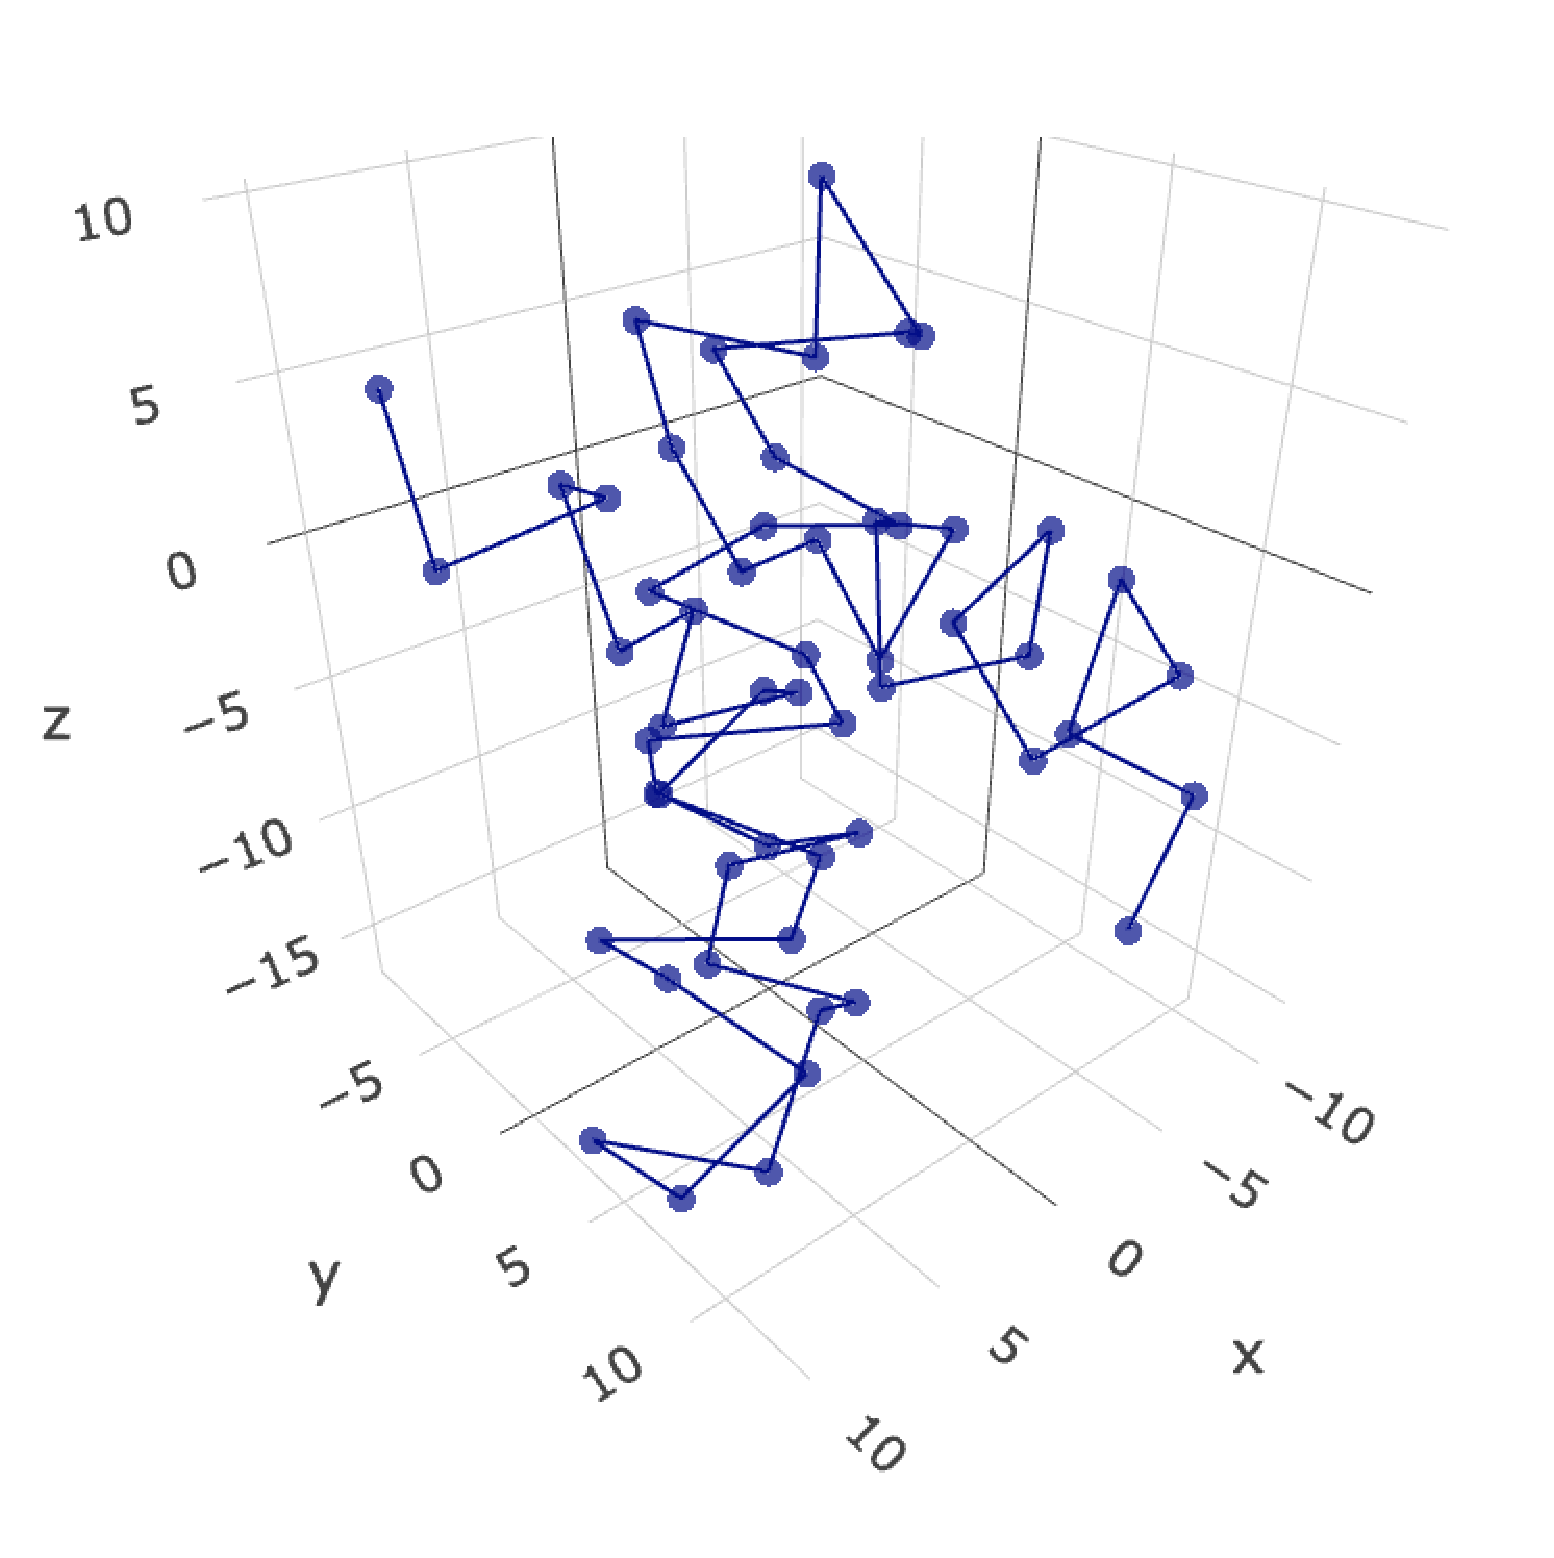
\includegraphics[width=\textwidth]{fig1.pdf}
					\caption{3D структура белка}
				\end{minipage}
				\hfill
				\begin{minipage}[b]{0.45\textwidth}
					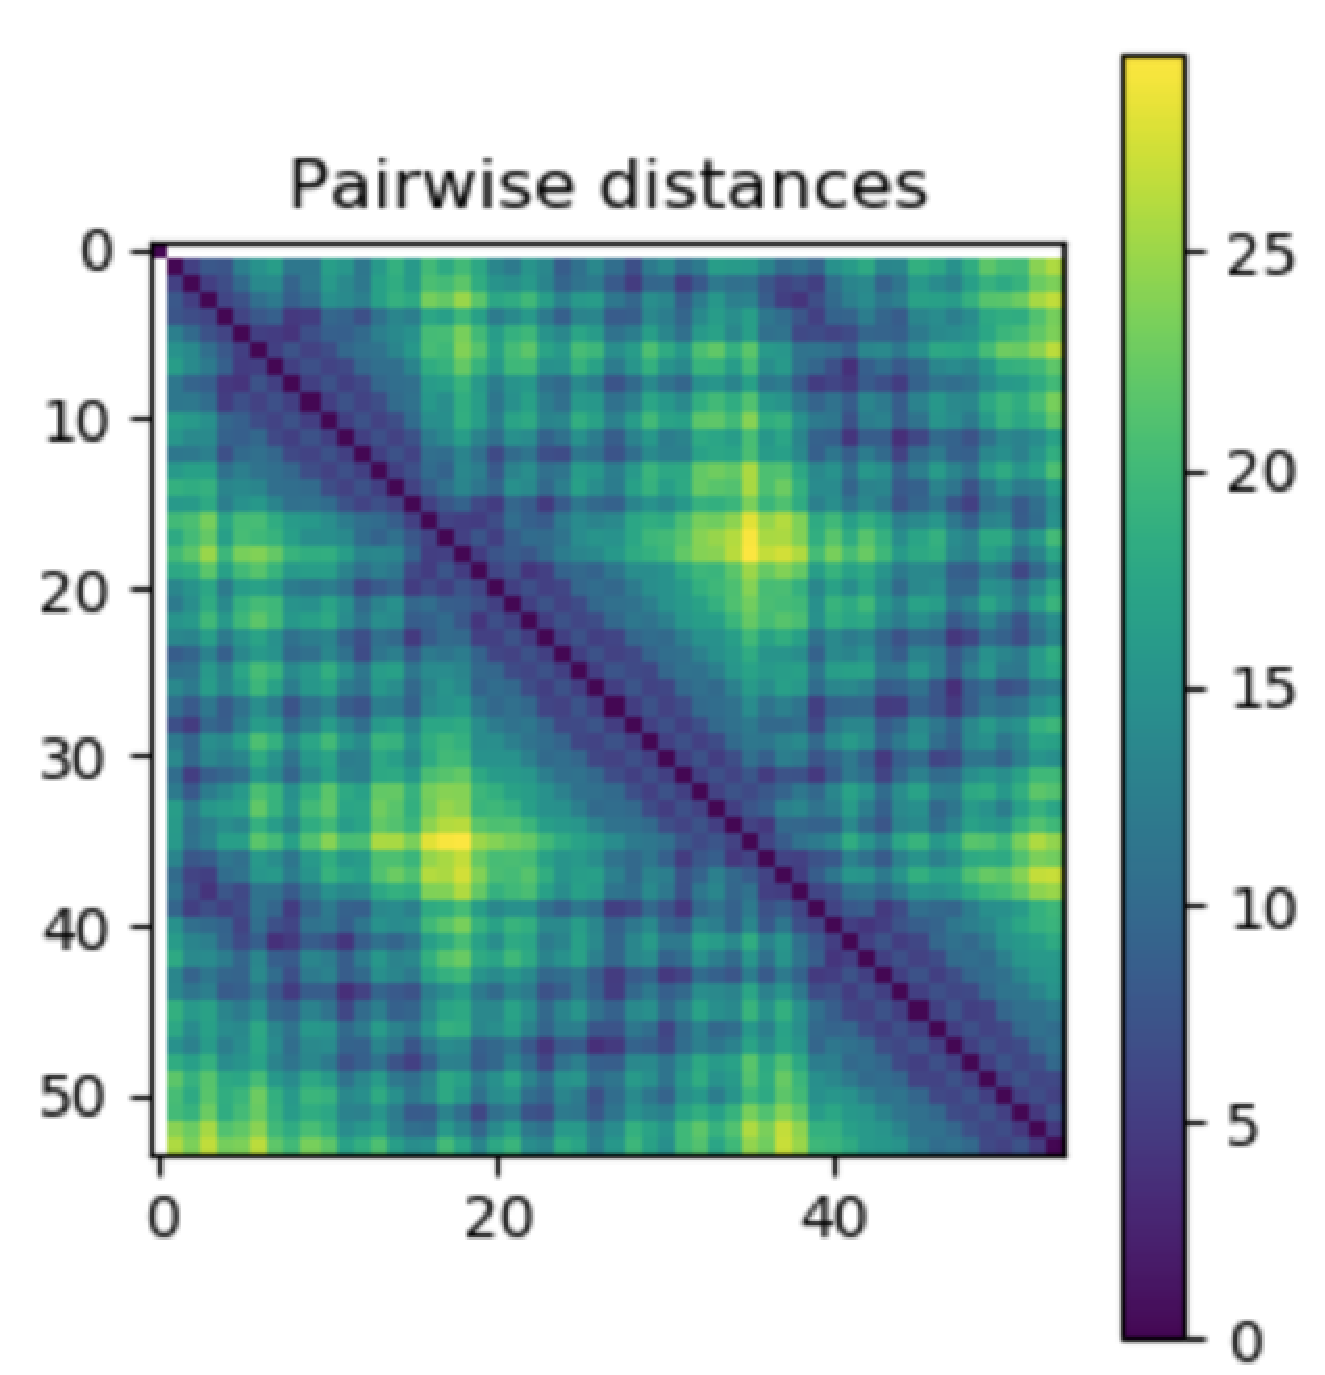
\includegraphics[width=\textwidth]{fig2.pdf}
					\caption{Попарные расстояния между элементами белка}
				\end{minipage}
			\end{figure}

			
			\subsection{Архитектуры сетей}
				\begin{enumerate}
					\item Deep Graph Convolutional Neural Network (DGCNN)\cite{Zhang2018AnED}
					\item 
					\item 
				\end{enumerate}
	
	\section{Результаты}
	
	
	

	\bibliographystyle{plain}
	\nocite{*}
	\bibliography{Severilov2019NIR}
	
\end{document}
